\documentclass[tikz,border=7pt]{standalone}
\usepackage{amsmath}
\usetikzlibrary{arrows.meta,calc,positioning,decorations.pathreplacing}
\definecolor{frameblue}{RGB}{42,66,167}
\definecolor{headerfill}{RGB}{238,242,252}
\definecolor{activefill}{RGB}{210,235,250}
\definecolor{activedraw}{RGB}{0,137,225}
\definecolor{ghostfill}{RGB}{222,228,236}
\definecolor{ghostdraw}{RGB}{145,154,168}
\definecolor{depthfill}{RGB}{249,221,187}
\definecolor{depthdraw}{RGB}{216,108,19}
\definecolor{tempfill}{RGB}{229,210,252}
\definecolor{tempdraw}{RGB}{119,45,205}
\tikzset{
  panel/.style={draw=frameblue, rounded corners=4pt, line width=0.9pt},
  header/.style={draw=frameblue, fill=headerfill, rounded corners=4pt, line width=0.9pt},
  sideheader/.style={draw=frameblue, fill=headerfill, rounded corners=4pt, line width=0.9pt},
  active/.style={draw=activedraw, fill=activefill, rounded corners=2pt, minimum width=1.15cm, minimum height=0.43cm, inner sep=0pt, line width=0.85pt},
  ghost/.style={draw=ghostdraw, fill=ghostfill, fill opacity=0.40, draw opacity=0.58, rounded corners=2pt, minimum width=1.15cm, minimum height=0.43cm, inner sep=0pt, line width=0.75pt},
  depthcell/.style={draw=depthdraw, fill=depthfill, rounded corners=2pt, minimum width=1.15cm, minimum height=0.43cm, inner sep=0pt, line width=0.95pt},
  tempcell/.style={draw=tempdraw, fill=tempfill, rounded corners=2pt, minimum width=1.15cm, minimum height=0.43cm, inner sep=0pt, line width=0.95pt},
  ghostdepth/.style={draw=depthdraw, fill=depthfill, fill opacity=0.28, draw opacity=0.55, rounded corners=2pt, minimum width=1.15cm, minimum height=0.43cm, inner sep=0pt, line width=0.90pt},
  ghosttemp/.style={draw=tempdraw, fill=tempfill, fill opacity=0.28, draw opacity=0.55, rounded corners=2pt, minimum width=1.15cm, minimum height=0.43cm, inner sep=0pt, line width=0.90pt},
  injectD/.style={circle, draw=depthdraw, fill=depthfill, minimum size=3.6mm, inner sep=0pt, line width=0.85pt, font=\bfseries\scriptsize},
  injectT/.style={circle, draw=tempdraw, fill=tempfill, minimum size=3.6mm, inner sep=0pt, line width=0.85pt, font=\bfseries\scriptsize},
  stateT/.style={draw=tempdraw, fill=tempfill, rounded corners=2pt, minimum width=1.15cm, minimum height=0.44cm, inner sep=1pt, line width=0.9pt, font=\scriptsize},
  stateD/.style={draw=depthdraw, fill=depthfill, rounded corners=2pt, minimum width=1.15cm, minimum height=0.44cm, inner sep=1pt, line width=0.9pt, font=\scriptsize},
  flow/.style={-{Latex[length=1.8mm]}, draw=black, line width=0.82pt},
  ghostflow/.style={-{Latex[length=1.5mm]}, draw=black!38, line width=0.58pt},
  dread/.style={-{Latex[length=1.9mm]}, draw=depthdraw, dashed, line width=0.95pt},
  tread/.style={-{Latex[length=1.9mm]}, draw=tempdraw, dashed, line width=0.95pt},
  descbox/.style={draw=frameblue!55, fill=white, rounded corners=2.5pt, line width=0.6pt, inner sep=1.6pt, align=center, font=\scriptsize},
  stage/.style={anchor=east,font=\scriptsize,align=right,text width=1.8cm},
  tinylabel/.style={font=\scriptsize,align=center},
}
\begin{document}
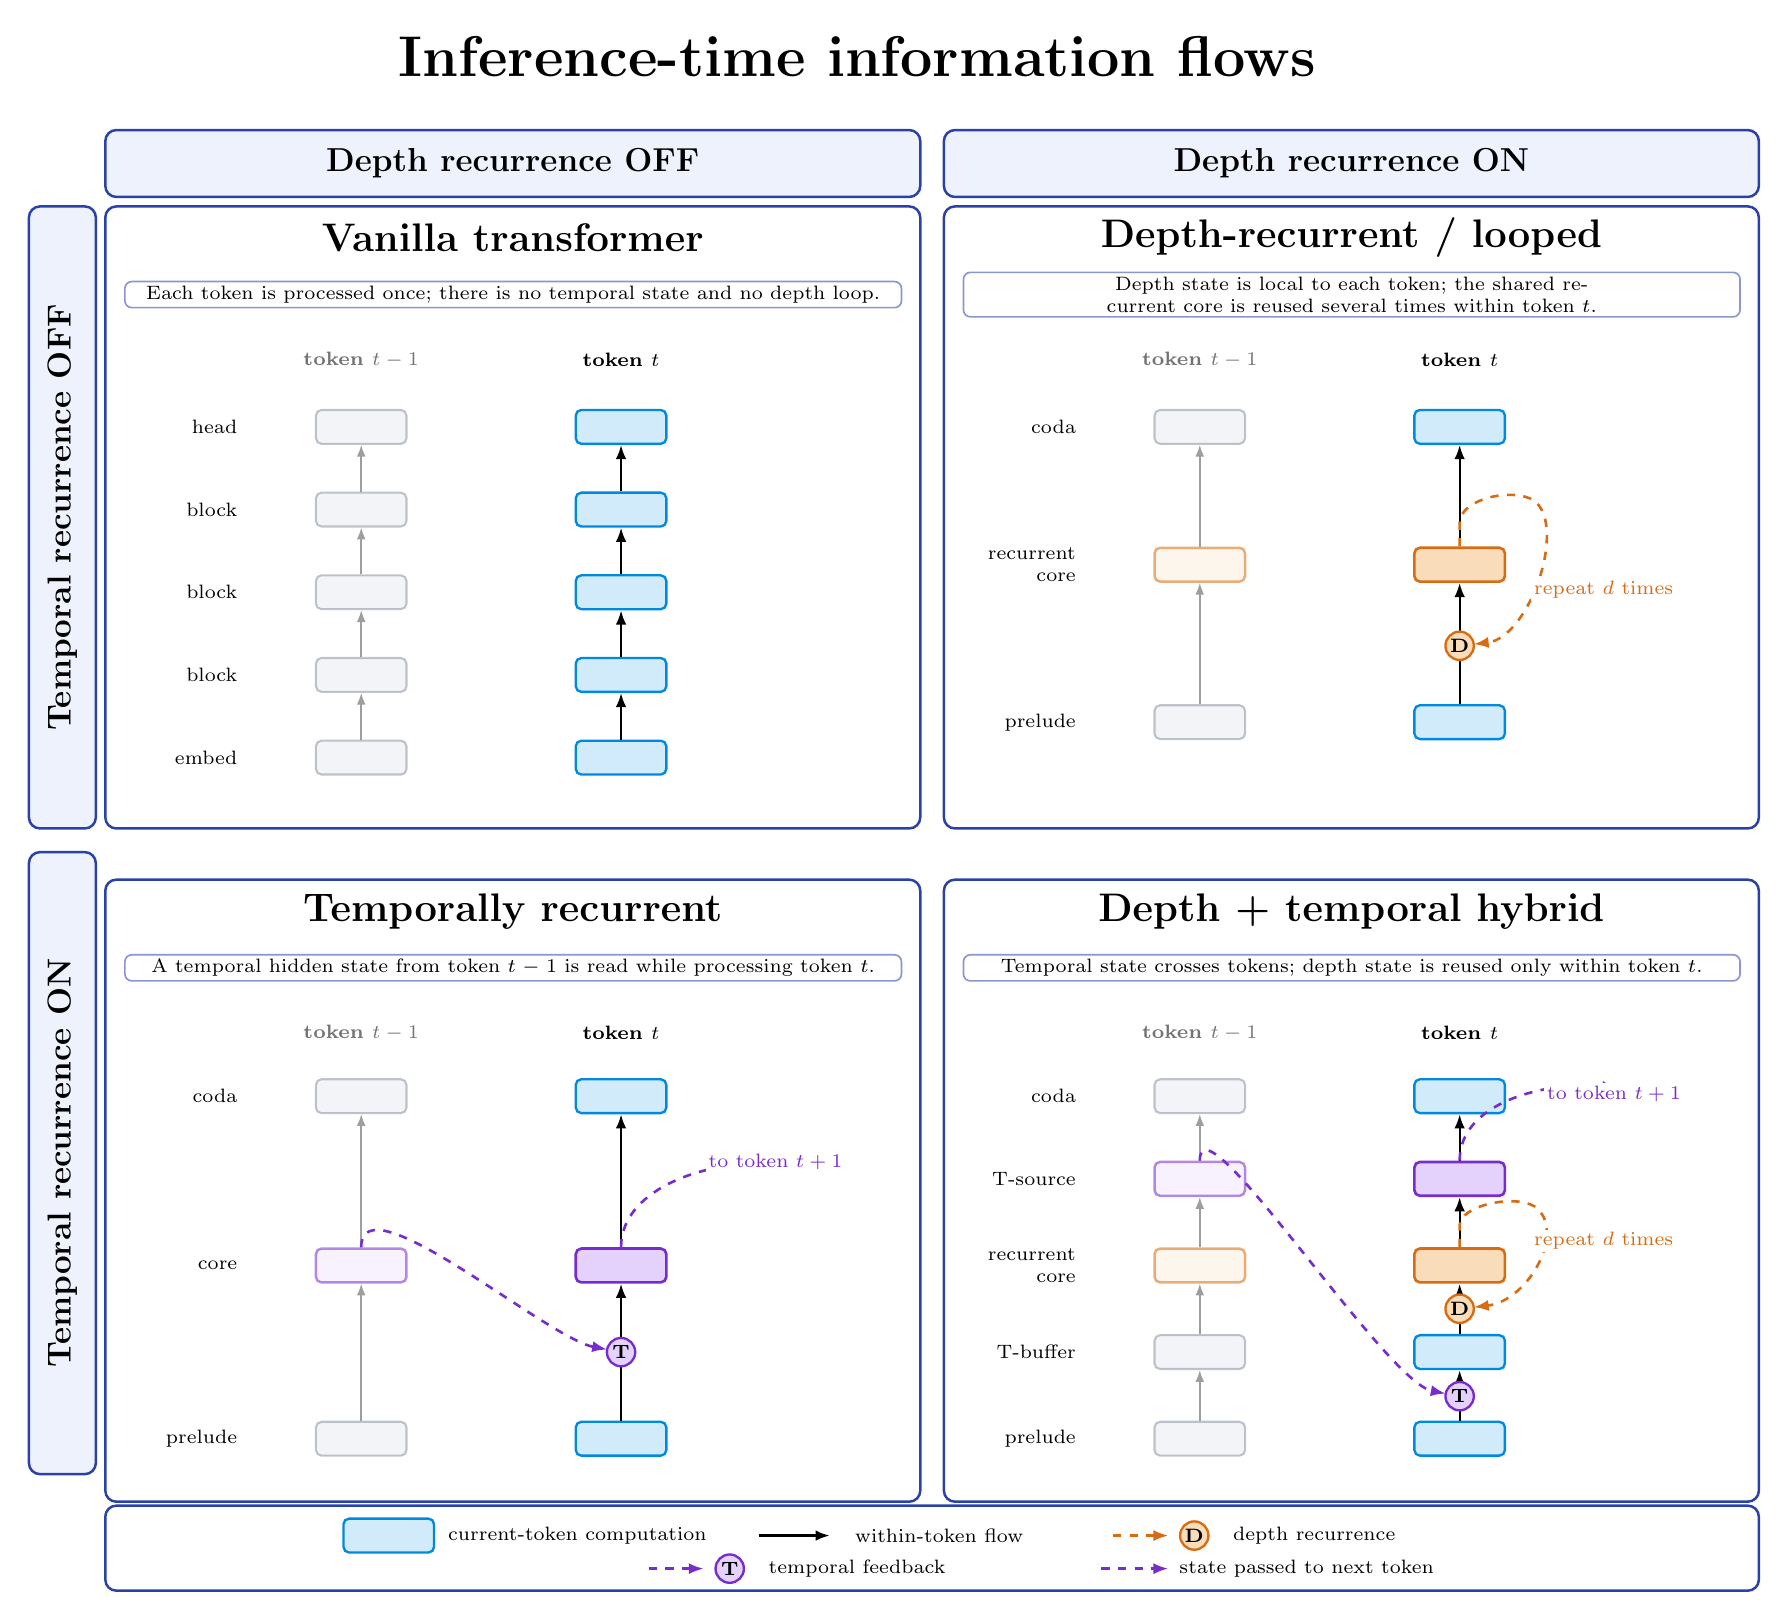
\begin{tikzpicture}[x=1cm,y=1cm]

\node[font=\bfseries\huge] at (11.9,17.30) {Inference-time information flows};
\node[header, minimum width=10.35cm, minimum height=0.85cm, font=\bfseries\large] at (7.525,15.945) {Depth recurrence OFF};
\node[header, minimum width=10.35cm, minimum height=0.85cm, font=\bfseries\large] at (18.175,15.945) {Depth recurrence ON};
\node[sideheader, minimum width=7.90cm, minimum height=0.85cm, rotate=90, font=\bfseries\large] at (1.805,11.45) {Temporal recurrence OFF};
\node[sideheader, minimum width=7.90cm, minimum height=0.85cm, rotate=90, font=\bfseries\large] at (1.805,3.25) {Temporal recurrence ON};

\begin{scope}[shift={(2.35,7.50)}]
  \draw[panel] (0,0) rectangle (10.35,7.90);
  \node[font=\bfseries\Large] at (5.175,7.50) {Vanilla transformer};
  \node[descbox,text width=9.75cm] at (5.18,6.78) {Each token is processed once; there is no temporal state and no depth loop.};
  \node[font=\bfseries\scriptsize,text=black!55] at (3.25,5.95) {token $t-1$};
  \node[font=\bfseries\scriptsize] at (6.55,5.95) {token $t$};
  \node[stage] at (1.80,5.10) {head};
  \node[stage] at (1.80,4.05) {block};
  \node[stage] at (1.80,3.00) {block};
  \node[stage] at (1.80,1.95) {block};
  \node[stage] at (1.80,0.90) {embed};
  % token t-1 (faded)
  \foreach \N/\Y in {a/0.90,b/1.95,c/3.00,d/4.05,e/5.10}{\node[ghost] (vg\N) at (3.25,\Y) {};}
  \draw[ghostflow] (vga.north)--(vgb.south); \draw[ghostflow] (vgb.north)--(vgc.south); \draw[ghostflow] (vgc.north)--(vgd.south); \draw[ghostflow] (vgd.north)--(vge.south);
  % token t (active)
  \foreach \N/\Y in {a/0.90,b/1.95,c/3.00,d/4.05,e/5.10}{\node[active] (v\N) at (6.55,\Y) {};}
  \draw[flow] (va.north)--(vb.south); \draw[flow] (vb.north)--(vc.south); \draw[flow] (vc.north)--(vd.south); \draw[flow] (vd.north)--(ve.south);
\end{scope}


\begin{scope}[shift={(13.00,7.50)}]
  \draw[panel] (0,0) rectangle (10.35,7.90);
  \node[font=\bfseries\Large] at (5.175,7.50) {Depth-recurrent / looped};
  \node[descbox,text width=9.75cm] at (5.18,6.78) {Depth state is local to each token; the shared recurrent core is reused several times within token $t$.};
  \node[font=\bfseries\scriptsize,text=black!55] at (3.25,5.95) {token $t-1$};
  \node[font=\bfseries\scriptsize] at (6.55,5.95) {token $t$};
  \node[stage] at (1.80,5.10) {coda};
  \node[stage] at (1.80,3.35) {recurrent\\core};
  \node[stage] at (1.80,1.35) {prelude};
  % token t-1 (faded)
  \node[ghost]      (dgp) at (3.25,1.35) {};
  \node[ghostdepth] (dgc) at (3.25,3.35) {};
  \node[ghost]      (dgo) at (3.25,5.10) {};
  \draw[ghostflow] (dgp.north)--(dgc.south);
  \draw[ghostflow] (dgc.north)--(dgo.south);
  % token t (active)
  \node[active]    (dap) at (6.55,1.35) {};
  \node[depthcell] (dac) at (6.55,3.35) {};
  \node[active]    (dao) at (6.55,5.10) {};
  \coordinate (dDpos) at (6.55,2.32);
  \draw[flow] (dap.north) -- (dac.south);
  \draw[flow] (dac.north) -- (dao.south);
  \draw[dread,shorten >=1.8mm]
    (dac.north) -- ++(0,0.30)
    .. controls +(0,0.30) and +(-0.28,0.18) .. ($(dac.north)+(0.95,0.58)$)
    .. controls +(0.42,-0.34) and +(0.88,0.10) .. (dDpos);
  \node[font=\scriptsize,text=depthdraw,align=left,fill=white,inner sep=1pt] at (8.38,3.03) {repeat $d$ times};
  % Injection marker is deliberately drawn last so it sits above the flow line.
  \node[injectD] at (dDpos) {D};
\end{scope}


\begin{scope}[shift={(2.35,-1.05)}]
  \draw[panel] (0,0) rectangle (10.35,7.90);
  \node[font=\bfseries\Large] at (5.175,7.50) {Temporally recurrent};
  \node[descbox,text width=9.75cm] at (5.18,6.78) {A temporal hidden state from token $t-1$ is read while processing token $t$.};
  \node[font=\bfseries\scriptsize,text=black!55] at (3.25,5.95) {token $t-1$};
  \node[font=\bfseries\scriptsize] at (6.55,5.95) {token $t$};
  \node[stage] at (1.80,5.15) {coda};
  \node[stage] at (1.80,3.00) {core};
  \node[stage] at (1.80,0.80) {prelude};
  % token t-1 (faded)
  \node[ghost]     (tgp) at (3.25,0.80) {};
  \node[ghosttemp] (tgc) at (3.25,3.00) {};
  \node[ghost]     (tgo) at (3.25,5.15) {};
  \draw[ghostflow] (tgp.north)--(tgc.south);
  \draw[ghostflow] (tgc.north)--(tgo.south);
  % token t (active)
  \node[active]    (tap) at (6.55,0.80) {};
  \node[tempcell]  (tac) at (6.55,3.00) {};
  \node[active]    (tao) at (6.55,5.15) {};
  \coordinate (tTpos) at (6.55,1.90);
  \draw[flow] (tap.north) -- (tac.south);
  \draw[flow] (tac.north)--(tao.south);
  \draw[tread,shorten >=1.8mm] (tgc.north) .. controls +(0,0.88) and +(-0.95,0.18) .. (tTpos);
  \draw[tread] (tac.north) .. controls +(0,0.78) and +(-0.80,0.10) .. (8.55,4.25);
  \node[anchor=west,font=\scriptsize,text=tempdraw,fill=white,inner sep=1pt] at (7.62,4.32) {to token $t+1$};
  % Injection marker is deliberately drawn last so it sits above the flow line.
  \node[injectT] at (tTpos) {T};
\end{scope}

\begin{scope}[shift={(13.00,-1.05)}]
  \draw[panel] (0,0) rectangle (10.35,7.90);
  \node[font=\bfseries\Large] at (5.175,7.50) {Depth + temporal hybrid};
  \node[descbox,text width=9.75cm] at (5.18,6.78) {Temporal state crosses tokens; depth state is reused only within token $t$.};
  \node[font=\bfseries\scriptsize,text=black!55] at (3.25,5.95) {token $t-1$};
  \node[font=\bfseries\scriptsize] at (6.55,5.95) {token $t$};
  \node[stage] at (1.80,5.15) {coda};
  \node[stage] at (1.80,4.10) {T-source};
  \node[stage] at (1.80,3.00) {recurrent\\core};
  \node[stage] at (1.80,1.90) {T-buffer};
  \node[stage] at (1.80,0.80) {prelude};
  % token t-1 (faded)
  \node[ghost]      (hgp) at (3.25,0.80) {};
  \node[ghost]      (hgb) at (3.25,1.90) {};
  \node[ghostdepth] (hgc) at (3.25,3.00) {};
  \node[ghosttemp]  (hgs) at (3.25,4.10) {};
  \node[ghost]      (hgo) at (3.25,5.15) {};
  \draw[ghostflow] (hgp.north)--(hgb.south);
  \draw[ghostflow] (hgb.north)--(hgc.south);
  \draw[ghostflow] (hgc.north)--(hgs.south);
  \draw[ghostflow] (hgs.north)--(hgo.south);
  % token t (active)
  \node[active]     (hap) at (6.55,0.80) {};
  \node[active]     (hab) at (6.55,1.90) {};
  \node[depthcell]  (hac) at (6.55,3.00) {};
  \node[tempcell]   (has) at (6.55,4.10) {};
  \node[active]     (hao) at (6.55,5.15) {};
  \coordinate (hTpos) at (6.55,1.34);
  \coordinate (hDpos) at (6.55,2.45);
  \draw[flow] (hap.north) -- (hab.south);
  \draw[flow] (hab.north) -- (hac.south);
  \draw[flow] (hac.north)--(has.south);
  \draw[flow] (has.north)--(hao.south);
  \draw[tread,shorten >=1.8mm] (hgs.north) .. controls +(0,0.88) and +(-0.95,0.18) .. (hTpos);
  \draw[dread,shorten >=1.8mm]
    (hac.north) -- ++(0,0.28)
    .. controls +(0,0.24) and +(-0.28,0.16) .. ($(hac.north)+(0.95,0.52)$)
    .. controls +(0.42,-0.30) and +(0.88,0.10) .. (hDpos);
  \node[font=\scriptsize,text=depthdraw,align=left,fill=white,inner sep=1pt] at (8.38,3.31) {repeat $d$ times};
  \draw[tread] (has.north) .. controls +(0,0.78) and +(-0.80,0.10) .. (8.55,5.25);
  \node[anchor=west,font=\scriptsize,text=tempdraw,fill=white,inner sep=1pt] at (7.62,5.18) {to token $t+1$};
  % Injection markers are deliberately drawn last so they sit above the flow lines.
  \node[injectT] at (hTpos) {T};
  \node[injectD] at (hDpos) {D};
\end{scope}

\begin{scope}[shift={(2.35,-2.18)}]
  \draw[panel] (0,0) rectangle (21.00,1.08);
  \begin{scope}[xshift=3.05cm]
    \node[active] at (0.55,0.70) {};
    \node[anchor=west,font=\scriptsize] at (1.18,0.70) {current-token computation};
    \draw[flow] (5.25,0.70) -- (6.15,0.70);
    \node[anchor=west,font=\scriptsize] at (6.35,0.70) {within-token flow};
    \draw[dread] (9.75,0.70) -- (10.45,0.70);
    \node[injectD] at (10.78,0.70) {D};
    \node[anchor=west,font=\scriptsize] at (11.15,0.70) {depth recurrence};
  \end{scope}
  \begin{scope}[xshift=6.65cm]
    \draw[tread] (0.25,0.28) -- (0.95,0.28);
    \node[injectT] at (1.28,0.28) {T};
    \node[anchor=west,font=\scriptsize] at (1.65,0.28) {temporal feedback};
    \draw[tread] (6.00,0.28) -- (6.85,0.28);
    \node[anchor=west,font=\scriptsize,fill=white,inner sep=1pt] at (6.95,0.28) {state passed to next token};
  \end{scope}
\end{scope}
\end{tikzpicture}
\end{document}
